\documentclass[11pt,a4paper,oneside]{report}
\usepackage[margin=25mm,footskip=11mm,headheight=14pt]{geometry}
\usepackage[T1]{fontenc}
\usepackage{helvet}
\usepackage{graphicx,booktabs,tabularx,array,caption,xcolor,listings,amsmath}
\usepackage[hidelinks]{hyperref}
\renewcommand{\familydefault}{\sfdefault}
\renewcommand{\contentsname}{Table of Contents}
\setlength{\parindent}{0pt}
\setlength{\parskip}{.65em}
\setlength{\emergencystretch}{2em}
\linespread{1.17}
\setcounter{tocdepth}{1}
\graphicspath{{assets/}}
\captionsetup{font=small,labelfont=bf,hypcap=false}
\definecolor{ink}{HTML}{1B3441}
\definecolor{papergray}{HTML}{F3F5F7}
\definecolor{good}{HTML}{21694C}
\definecolor{warn}{HTML}{9C4934}
\lstset{basicstyle=\ttfamily\small,backgroundcolor=\color{papergray},frame=single,rulecolor=\color{black!18},columns=fullflexible,breaklines=true,breakautoindent=false,breakindent=14pt,keepspaces=true,showstringspaces=false,xleftmargin=6pt,xrightmargin=6pt,aboveskip=7pt,belowskip=7pt}
\hypersetup{pdftitle={SentinelAPI - Information Security Project Report},
  pdfauthor={Soham Agarwal, Aayush Doshi, Divyam Khandelwal, Prem Sharma}}
\makeatletter
\def\ps@sentinel{%
  \def\@oddhead{\small SentinelAPI\hfill Information Security Project Report}%
  \let\@evenhead\@oddhead
  \def\@oddfoot{\hfil\thepage\hfil}%
  \let\@evenfoot\@oddfoot}
\renewcommand{\@makechapterhead}[1]{%
  {\centering\parindent\z@\normalfont\Large\bfseries
    Chapter \thechapter: #1\par\nobreak\vskip 18pt}}
\renewcommand{\@makeschapterhead}[1]{%
  {\centering\parindent\z@\normalfont\Large\bfseries #1\par\nobreak\vskip 18pt}}
\makeatother
\newcommand{\ProjectTitle}{SentinelAPI}
\newcommand{\ProjectSubtitle}{Local Security Testing and Intrusion Detection Lab}
\newcommand{\Course}{IT305 Information Security}
\newcommand{\Supervisor}{Dr Pooja Mishra}
\newcommand{\AcademicYear}{2026--27}
\newcommand{\Institute}{Indian Institute of Information Technology Vadodara}
\newcommand{\Department}{Department of CSE}
\newcommand{\TeamRows}{Soham Agarwal & 202452332\\Aayush Doshi & 202452301\\Divyam Khandelwal & 202452316\\Prem Sharma & 202452328\\}
\newcommand{\topic}[1]{\par\addvspace{4pt}\noindent\textbf{#1}\par\nobreak\vspace{-.20em}}
\newcommand{\casecode}[1]{\texttt{#1}}
\newcommand{\sheet}[1]{\clearpage\section{#1}}
\newcommand{\tabletitle}[1]{\par\addvspace{6pt}\noindent\parbox{\linewidth}{\captionof{table}{#1}}\par\nobreak}
\newcolumntype{Y}{>{\raggedright\arraybackslash}X}
\newcommand{\bodytable}[1]{\begin{tabularx}{\linewidth}{@{}>{\raggedright\arraybackslash}p{.25\linewidth}Y@{}}\toprule #1\bottomrule\end{tabularx}}
\newcommand{\callout}[1]{\noindent\colorbox{papergray}{\parbox{\dimexpr\linewidth-2\fboxsep\relax}{\small\strut #1\strut}}}
\newcommand{\diagram}[1]{\begin{center}\footnotesize #1\end{center}}
\newcommand{\nodebox}[1]{\fbox{\strut #1}}
\newcommand{\arr}{\ \(\longrightarrow\)\ }
\begin{document}
\begin{titlepage}
\centering
\vspace*{5mm}

\includegraphics[width=.70\textwidth]{institute-masthead.png}\par
\vspace{9mm}
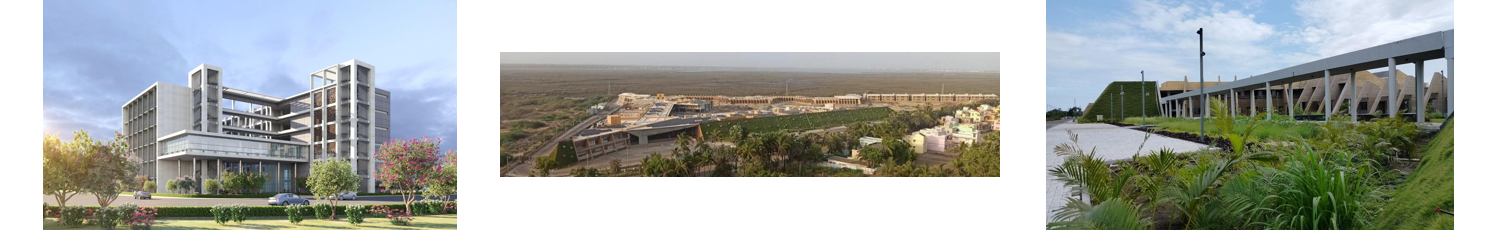
\includegraphics[width=.96\textwidth]{campus-strip.png}\par

\vspace{12mm}
{\Large\bfseries Information Security Project Report\par}
\vspace{8mm}
{\LARGE\bfseries\ProjectTitle\par}
\vspace{4mm}
{\large\bfseries\ProjectSubtitle\par}
\vspace{9mm}
{\large\bfseries\Course\par}
\vspace{4mm}
{\large\bfseries \Department\\Academic Year \AcademicYear\par}

\vfill
\begin{minipage}[t]{.59\linewidth}
\raggedright\textbf{Submitted By}\par\medskip
\renewcommand{\arraystretch}{1.2}%
\begin{tabular}{@{}ll@{}}\TeamRows\end{tabular}
\end{minipage}%
\begin{minipage}[t]{.40\linewidth}
\centering\textbf{Under the Guidance of}\par\medskip
\Supervisor
\end{minipage}
\vspace{8mm}
\end{titlepage}

\pagenumbering{arabic}
\setcounter{page}{2}
\chapter*{CERTIFICATE}
\phantomsection\addcontentsline{toc}{chapter}{Certificate}
\begin{center}

\includegraphics[width=28mm,trim=150 150 150 150,clip]{iiitlogo.png}\\[3mm]
\textbf{\Institute}\\
\Department
\end{center}
\vspace{4mm}
This is to certify that the following students prepared the project report entitled
\emph{\ProjectTitle: \ProjectSubtitle} as part of the academic requirements for
\Course\ in the academic year \AcademicYear.

The report documents the project design, implementation, and evaluation. The sources and external materials used in the project are acknowledged in the references.

\medskip
\textbf{Group Number}\quad\rule{2.35in}{.4pt}

\medskip
\textbf{Team Members}
\begin{center}
\renewcommand{\arraystretch}{1.3}%
\begin{tabular}{@{}p{.51\linewidth}p{.26\linewidth}@{}}
\toprule
\textbf{Name} & \textbf{Roll Number}\\
\midrule
\TeamRows
\bottomrule
\end{tabular}
\end{center}
\bigskip
\textbf{Project Supervisor}\quad \Supervisor

\vspace{.75in}
\textbf{Signature of Supervisor}\quad\rule{2.3in}{.4pt}

\textbf{Date}\quad\rule{2.3in}{.4pt}

\chapter*{Abstract}
\phantomsection\addcontentsline{toc}{chapter}{Abstract}
SentinelAPI is a local lab for testing how a web API responds to suspicious and ordinary requests. Express middleware applies seven signature detectors and four behavioral checks. The React dashboard shows the HTTP response, the rule or counter behind it, and any linked alert. PostgreSQL stores the experiment results and investigation records.

The simulator sends each case to the authenticated local API and compares the actual status and linked alert with the case's expected result. The demo handlers treat submitted input as data. In an archived Standard run, all 175 cases met their expectations: 62 returned 200, 8 returned 401, 78 returned 403, 15 returned 404, and 12 returned 429. A separate Extended run, limited to SQL injection and cross-site scripting (XSS), matched 106 of 142 expectations. The expected detector was missing in the other 36 cases. A later run passed all 12 normal-traffic controls.

On 21 labeled search inputs, the current SQL rule corrected six decisions made by a practice rule that flags any apostrophe. Five suspicious inputs were flagged and one ordinary surname was allowed. No case changed from correct to incorrect. The incident timeline records what an analyst did after an alert. A keyed audit chain verified new records and detected an edit and a deletion in a disposable sample. The latest build, lint, and 12 automated tests passed. The results describe the cases examined in the lab.

\textbf{Keywords:} application-layer intrusion detection, API security, signature matching, rate limiting, false positives, incident triage, tamper-evident audit.

\tableofcontents
\clearpage
\pagestyle{sentinel}
\setlength{\extrarowheight}{2pt}
\AddToHook{env/tabularx/before}{\noindent}
\AddToHook{env/tabularx/after}{\par\addvspace{6pt}}
\captionsetup[table]{skip=6pt,position=above}

\chapter{Introduction}
\section{Background and context}
A web API reads values from URLs, bodies, headers, and uploaded files. It also sees requests in sequence, which matters when no individual request is unusual. An apostrophe in a search term illustrates the problem with a rule that simply flags punctuation: it could block a perfectly ordinary surname.

Detection records a finding. Prevention changes how the request is handled. NIST distinguishes these functions in its guide to intrusion detection and prevention systems \cite{nist}. In this lab, repeated visits to missing routes can raise an alert while the API continues to return 404. Other rules can reject a request with 403 or enforce a temporary limit with 429.

The operator starts a case from the dashboard. A worker sends it to the local API, compares the response with the case plan, and links any alert to the result. An analyst can then review the alert and see that action in the incident timeline.

\topic{Why the application layer matters}
Express gives the middleware access to parsed fields, headers, and uploaded file buffers. A detector can identify which field it checked or which counter reached a limit. The project operates at the HTTP application layer; it does not capture raw packets.

\topic{Information security goals}
The file and destination checks illustrate confidentiality risks. The injection examples relate to unauthorized changes or execution. The flood case tests availability by checking whether ordinary requests work again after cooldown. Audit verification gives a separate example of integrity: it tests whether signed records agree with the checkpoint.

\sheet{Problem, aim and objectives}
\topic{Problem statement}
A 403 reply does not tell a reviewer which control refused the request. A 404 can be an ordinary missing route even when a series of 404s triggers an alert. The project needs enough evidence to answer two questions for each case: what did the API return, and what did its detectors record?

\topic{Aim}
Build a rule-based API security lab whose cases can be repeated and whose decisions and reviews can be inspected.

\topic{Objectives}
\begin{enumerate}
\item Inspect selected query, body, header, path, and upload inputs before application processing.
\item Track selected behavioral patterns within bounded time windows.
\item Provide controlled experiments with suspicious cases and normal-traffic controls.
\item Compare the actual response and persisted detector identity with the expected result for each case.
\item Explain decisions using a rule identifier, the inspected field, and measured counters where available.
\item Support incident review and verification of newly signed audit events.
\end{enumerate}

\topic{Acceptance example}
A normal search passes when it returns 200 with no linked alert. A signature case that expects 403 also requires an alert from the named detector. For a threshold case, the expected result changes at a specified point in the sequence.

\callout{The unit of evaluation is a defined test case with explicit expectations. Each expectation is interpreted in the context of the scenario and its position in the sequence.}

\sheet{Scope and report structure}
A student can open one case and follow it from the submitted field or rate counter to the detector decision and the analyst's review. The rule comparison provides a second way to study the same problem: it shows which fixed search cases change outcome when the SQL rule changes.

\tabletitle{Scope of the project}
\bodytable{\textbf{Area} & \textbf{Included work}\\\midrule
Inspection & HTTP request signatures and short behavioral windows.\\
Experimentation & Predefined local scenarios, normal controls, Extended inputs, and selected custom inputs.\\
Analyst workflow & Alert states, review verdicts, incident timelines, role and ownership restrictions.\\
Evidence & Saved experiment results, exports, audit records, and verification for signed events.\\
Evaluation & Recorded lab runs, a fixed comparison set, automated tests, and isolated database checks.\\}
\par

The local handlers do not execute submitted SQL, browser scripts, or shell text, and the fetch endpoint does not make an outbound request. Counters are held in one backend process. The audit check relies on a protected signing key and a checkpoint from the expected database state.

\topic{Organisation of the report}
Chapters 2 through 4 explain the sources, design, setup, and test data. Chapter 5 follows the request through the implementation and includes code excerpts. Chapters 6 and 7 explain the evaluation and its results. Chapter 8 describes the demonstration and the remaining work.

\medskip
\tabletitle{Abbreviations used in the report}
\begin{tabularx}{\linewidth}{@{}lYlY@{}}\toprule
API & Application programming interface & JWT & JSON Web Token\\
IDS & Intrusion detection system & SSE & Server-sent events\\
IPS & Intrusion prevention system & SSRF & Server-side request forgery\\
XSS & Cross-site scripting & HMAC & Hash-based message authentication code\\
\bottomrule\end{tabularx}

\chapter{Literature Review}
\section{Signature and behavioral detection}
Scarfone and Mell distinguish signature detection, anomaly detection, and stateful protocol analysis \cite{nist}. That distinction helps explain why SentinelAPI can check one search value immediately but needs a sequence of observations to identify repeated failed logins.

A signature looks for a particular pattern. When a rule matches, SentinelAPI can show the request field and the rule name. The record describes what matched under the lab's parsing rules; it gives no estimate of the probability of compromise.

Behavioral rules count recent events within a defined scope. Repeated failures on one account and failures spread across several usernames need different counters. The lab chooses its windows to demonstrate both cases clearly.

\topic{Relationship to learning-based systems}
Some intrusion detection systems learn a profile from past traffic. SentinelAPI uses fixed rules and explicit limits, so there is no model or training dataset. The quality of the result depends on how well those rules and fixtures represent the request context.

\tabletitle{Two sources of detection evidence}
\bodytable{\textbf{Mechanism} & \textbf{Example evidence}\\\midrule
Signature & Name of the rule and the field or file element it evaluated.\\
Behavior & Measured count, threshold, observation window, and resulting HTTP decision.\\}

\sheet{Web security testing and case design}
The OWASP Web Security Testing Guide separates input validation, authentication, authorization, and session testing \cite{owasp}. We use the same distinction when reading the lab results. A failed login tests credential handling; an authenticated user trying to read another user's report tests authorization.

Bozic and Wotawa describe planning-based web testing with attack grammars \cite{bozic}. SentinelAPI separates the case catalog from the runner for a related reason: the catalog records what should happen, and the runner measures what actually happened. SentinelAPI executes a fixed local plan.

Brandi, Perrone, and Romano use a test oracle to interpret observations from a web fuzzer \cite{brandi}. Their work illustrates why seeing text in a response is insufficient evidence of execution. In SentinelAPI, a matching signature shows that the defense recognized a pattern in the request.

For each case the test oracle checks the response and any required alert. A benign control can also require no alert. If another rule returns the same status, the intended detector can still fail the test.

\topic{Positive and negative controls}
Positive controls establish whether recognizable suspicious input or behavior is detected. Negative controls establish whether valid input continues to work. A meaningful comparison must use the same cases for both rules and hold the expectations constant. The comparison of an apostrophe-only practice rule with the current SQL signature follows this approach.

\topic{Repeatability}
A saved run identifies the profile, case selection, and artifact time. Sequences that depend on timing also check the phase of each response. In the flood case, the recovery request is graded separately from requests sent during cooldown.

\sheet{Alert review and audit integrity}
An alert has a workflow state and a separate review verdict. For example, an analyst can mark an alert as a false positive and then resolve it. The final record still shows why it was resolved.

The incident timeline uses the run ID to group case events, alerts, and review actions. A reviewer can read the sequence from the start of the run through the last recorded status or verdict change.

The audit feature uses HMAC \cite{hmac}. Each signed event includes a tag that depends on the previous tag. The checkpoint records the last tag and the number of signed events. Editing an event breaks its tag; removing the last event leaves the remaining chain inconsistent with the checkpoint.

\tabletitle{Security decisions and evidence decisions}
\bodytable{\textbf{Decision} & \textbf{Question answered}\\\midrule
Request outcome & Did the API allow, reject, rate limit, or report the request?\\
Expectation outcome & Did this result meet the criteria specified by the case?\\
Analyst verdict & Does a reviewer consider the alert a confirmed detection or a false positive?\\
Audit integrity & Do the signed records match the saved checkpoint?\\}

Cryptographic verification depends on protecting the secret and retaining a trustworthy checkpoint. It does not label an analyst's verdict as correct. It verifies the recorded sequence within the selected signed range, including whether the records still agree with the chain produced by the application.

\sheet{How the references informed the project}
NIST describes detection and prevention functions, OWASP organizes web security tests, and the research papers offer examples of how to design or interpret security experiments. The table identifies the part of the project each reference informed.

\tabletitle{Relationship between references and project design}
\bodytable{\textbf{Reference} & \textbf{Relationship to SentinelAPI}\\\midrule
NIST IDPS guide \cite{nist} & Provides a framework for distinguishing detection and prevention. SentinelAPI applies the distinction at the HTTP application boundary.\\
OWASP WSTG \cite{owasp} & Helps separate input handling, authentication, and authorization tests.\\
Bozic and Wotawa \cite{bozic} & Motivates separating test descriptions from concrete execution and observations.\\
Brandi et al. \cite{brandi} & Treat the evidence interpretation and test oracle as explicit design decisions.\\
PenQuest \cite{penquest} & Connects attacker and defender behavior to security education.\\
Mirage \cite{mirage} & Highlights how the choice of experimental environment affects what can be concluded.\\
HTTP specifications \cite{http,rfc429} & Explain response semantics used when measuring and labeling outcomes.\\
HMAC specification \cite{hmac} & Supports the keyed authentication mechanism used for audit integrity verification.\\}

\topic{Project gap}
Showing that an API once returned 403 leaves two practical questions unanswered: would the same rule block an ordinary input, and which detector actually caused the rejection? The report pairs a comparison on labeled cases with evidence from the live middleware, so each question has a separate check.

PenQuest motivated the link between offensive behavior and defensive evidence in a teaching tool. Mirage illustrates why the experimental setting matters. In our case, the HTTP request reaches real middleware, and the endpoint returns a controlled response in place of the downstream operation.

\topic{Evaluation question}
The evaluation uses saved local runs, a fixed set of search inputs, and targeted review and integrity tests. It can show what happened in those experiments. It cannot estimate detection rates on enterprise traffic.


\chapter{Methodology and system design}
\section{System architecture}
The dashboard and terminal client call the Express API. A worker builds the case plan and sends requests back to the local API. The middleware decides whether each request reaches the controlled handler. PostgreSQL stores accounts, runs, alerts, and review activity.

\diagram{\nodebox{Dashboard or CLI}\arr\nodebox{Authenticated API}\arr\nodebox{Experiment worker}\\[8pt]
\nodebox{Loopback request}\arr\nodebox{Detector pipeline}\arr\nodebox{Controlled handler}\\[8pt]
\nodebox{HTTP response}\arr\nodebox{Verifier and database}\arr\nodebox{Result view}}
\noindent\parbox{\linewidth}{\captionof{figure}{SentinelAPI experiment architecture. Management calls configure the run; loopback requests carry individual cases.}}

\tabletitle{Major components and their responsibilities}
\bodytable{\textbf{Component} & \textbf{Responsibility}\\\midrule
React interface & Configure a scenario, inspect decision evidence, and navigate results.\\
Express API & Authenticate, validate options, dispatch routes, and return status.\\
Runner and catalog & Produce labeled cases, bind requests to a run, and verify the evidence.\\
Detector middleware & Inspect inputs and counters and make request-level decisions.\\
PostgreSQL & Persist account, run, alert, review, and audit information.\\}

Direct and simulated lab requests use the same middleware. The server accepts simulation metadata only if it identifies a registered active case belonging to the operator. A caller cannot choose a different counter scope by supplying arbitrary run headers.

\sheet{From request to saved result}
Management requests handle sign-in, configuration, progress, cancellation, and reports. The test requests carry active run and case IDs. Middleware validates that association before the simulation can use it to look up case-specific alerts.

\begin{enumerate}
\item The operator selects a scenario, profile, and optional settings in the playground.
\item The API evaluates role and configuration constraints and creates a run record.
\item The runner sends each defined case to the local API.
\item Middleware checks whether the request is in an active rate-limit window and applies the detectors in order.
\item The runner captures the actual response and reads the database evidence attributed to the case.
\item The verifier compares the observations with the expectation. The report is updated with progress and final state.
\end{enumerate}

\topic{Three independent observations}
The response is what the client received. The alert identifies what the detector recorded. The test result compares both with the case plan. A series of missing routes can correctly return 404 throughout and still raise an enumeration alert at the threshold.

\topic{Live alerts and saved evidence}
The live stream notifies the dashboard of alert changes. If that connection drops, saved reports remain available from the API. Replay steps through stored rows without issuing the original requests again.

\callout{A result can be reconstructed from the response status, required detector, and linked alert IDs. A color or result badge alone is insufficient evidence.}

\sheet{Trust boundaries and state isolation}
\topic{Authentication boundary}
Account sign-in checks database-backed credentials. The demo login route is a protected endpoint that returns controlled results for login-behavior cases. Calling it requires an authenticated lab operator.

\topic{Evidence ownership boundary}
The server checks both role and record ownership. Administrators can review evidence across accounts. Analysts can work with their own records, and viewers can read theirs. The labeled comparison fixtures are shared.

\topic{Detector state boundary}
The server groups ordinary observations by authenticated user and source. Simulated observations are grouped by run and lane. A lane holds related cases, such as the failures in one login sequence. Run completion or cancellation frees that temporary state.

\topic{Persistence boundary}
Counts and temporary limits remain in process memory. Alerts, reports, and review verdicts survive a restart through PostgreSQL. A restart can leave a run incomplete, so persisted progress remains useful even if the remaining requests were never executed.

\medskip
\tabletitle{Record relationships used by the investigation views}
\bodytable{\textbf{Record} & \textbf{Key relationship}\\\midrule
\texttt{users} & Account identity and role provide the ownership boundary.\\
\texttt{simulation\_runs} & Run ID identifies the experiment, owner, case results, and current lifecycle state.\\
\texttt{alerts} & Owner, run, and case identifiers connect a detection and its decision evidence to a request.\\
\texttt{audit\_events} & Actor and entity identifiers connect actions to runs or alerts.\\
\texttt{auth\_events} & Records account authentication activity separately from investigation actions.\\
Audit checkpoint & Stores the chain head and count used to verify the signed audit records.\\}

\sheet{HTTP outcomes and detector logic}
\tabletitle{Interpretation of HTTP outcomes within the lab}
\begin{tabularx}{\linewidth}{@{}lYY@{}}\toprule
\textbf{HTTP} & \textbf{Typical observation} & \textbf{Evidence interpretation}\\\midrule
200 & A controlled handler accepts a request. & A normal control expects no alert.\\
401 & Demo credentials are invalid. & An early failed attempt can meet its expectation.\\
403 & A request is refused. & The required detector record confirms an expected signature or behavior block.\\
404 & The requested lab route does not exist. & Repeated 404s can have an enumeration alert at the threshold.\\
429 & The request rate is limited. & A recorded threshold event explains the active cooldown.\\
503 & Inspection cannot be completed. & A service problem calls for investigation, not classification.\\
\bottomrule\end{tabularx}

HTTP status meanings follow the protocol semantics \cite{http,rfc429}. Scenario-specific interpretations depend on the context above. Management routes may also use these codes for their own authentication, access, or service decisions.

\topic{Signature checks}
The application extracts string values from selected request locations and normalizes common encodings before pattern matching. Field paths can be attached to a decision. Sensitive values are redacted in the structured matched-input evidence.

\topic{Behavioral checks}
A detector keeps recent timestamps or distinct identities for a specific scope. It discards observations outside the window. Reaching a threshold can emit an alert, block the current request, or set a cooldown depending on the rule.

\topic{Audit verification}
Audit events are ordered by database record ID. The verifier recomputes each authentication tag and then compares the final tag and count with a signed checkpoint. Verification is an administrative operation. The standalone demonstration changes a temporary copy of signed records.

\chapter{Tools and technologies}
\section{Languages, frameworks and libraries}
TypeScript is used across the backend, the dashboard, and the shared contracts. This lets request results and decision evidence use common field names between components. The runtime still verifies untrusted inputs because TypeScript annotations are removed during execution.

\tabletitle{Technologies and their roles}
\bodytable{\textbf{Technology} & \textbf{Role in the project}\\\midrule
Node.js and TypeScript & API execution, local client, shared data contracts, and automated tests.\\
Express & HTTP routing and input/detection middleware.\\
React and Vite & Dashboard state, navigation, inspection views, development server, and build.\\
PostgreSQL and \casecode{pg} & Persistent accounts, reports, alerts, reviews, and integrity checkpoint.\\
bcryptjs & Password hashing and verification.\\
jsonwebtoken & JWT creation and validation.\\
Multer & Multipart decoding and in-memory file buffers for upload inspection.\\
Node test and assert & Automated checks for detectors, reports, comparison, and audit integrity.\\
Oxlint & Frontend linting.\\}

\topic{Why this stack fits the project}
Shared TypeScript interfaces give an evidence object the same field names on the server and dashboard. PostgreSQL lets a review and its audit record commit together. The runner checks the response and stored data that the dashboard later reads.

\topic{Version reproducibility}
Install from the repository lockfiles. To verify a new installation, run the checks below. Archived measurements are listed with their run identifiers in Chapter 7.

\sheet{Local setup}
One developer laptop can run the API, dashboard, and test runner. The documented setup uses Node.js 22 or later, npm, a current browser, and PostgreSQL 16 on macOS. PostgreSQL 14 or later meets the stated database requirement.

\tabletitle{Local components and configuration}
\bodytable{\textbf{Component} & \textbf{Default or purpose}\\\midrule
API & \texttt{http://localhost:3000}; handles local HTTP and database work.\\
Dashboard & \texttt{http://localhost:5173}; connects through a configurable API URL.\\
Database & PostgreSQL with local database \texttt{sentinelapi}; configuration via \texttt{DATABASE\_URL}.\\
Frontend origin & Must agree with the URL used by the browser for cookies and live updates.\\
Audit key & Set \texttt{AUDIT\_INTEGRITY\_SECRET} before signing begins, or use the configured local fallback. Keep the original signing key available.\\}

\begin{lstlisting}[caption={Setup and verification commands from the repository root}]
npm ci
npm ci --prefix dashboard
npm run check

# Terminal 1, with PostgreSQL available
npm run dev

# Terminal 2
cd dashboard
npm run dev -- --host localhost --strictPort
\end{lstlisting}

The database must exist before starting the API on a fresh installation. The server adds its tables, indexes, and additive schema updates during startup. A health request verifies both server reachability and database connectivity. Existing data and configured local secrets should be retained between restarts.

\sheet{Test data and profiles}
The Standard profile contains project-defined suspicious inputs and ordinary traffic. Each line of evaluation is linked to a defined scenario and may specify a response code, detector, or absence of an alert. A separate set of community inputs broadens SQL and XSS coverage in the Extended profile.

\tabletitle{Test sets and their composition}
\bodytable{\textbf{Set} & \textbf{Composition}\\\midrule
Standard & 175 HTTP requests with the default 20 demo password attempts and all scenarios selected.\\
Full Extended & 295 planned HTTP requests, including 120 additional SQL and XSS probes.\\
Selected Extended & 142 SQL and XSS requests in the recorded two-family run.\\
Rule comparison & 21 fixed search fixtures evaluated offline by two rule definitions.\\
Normal traffic & 12 HTTP requests covering routine search, upload, login, and simulated fetch behavior.\\}

The community corpus is bundled from SecLists \cite{seclists}. The repository records the pinned revision, attribution, and license information. The bundled collection contains 1,000 common password entries, 268 generic SQL inputs, and 110 XSS inputs. Extended adds 60 inputs from each of the SQL and XSS collections to the Standard cases when those scenarios are selected.

\textbf{Corpus revision} \texttt{ab068333d7d44a9376e2037b0ed7d2e8ca5c6610}

\topic{Interpretation of an expected detector}
A missing alert means the detector named in the case did not appear. Some strings have meaning only in a particular query, browser, or interpreter context. The rules inspect the request as received, which limits what these cases can establish about exploitability.

\topic{Reproducibility}
The run ID, profile, selected scenario keys, input source, and expected decisions define what was measured. The chosen password count can change the size of a plan. Stored evidence redacts login passwords, so the report can be reviewed without reproducing raw credentials.

\addtocontents{toc}{\protect\newpage\protect\noindent\protect\textbf{Table of Contents (continued)}\protect\par\protect\medskip}
\chapter{Implementation}
\section{Backend and middleware}
Express parses and authenticates protected requests before handing them to the detectors. Management requests such as dashboard polling are separate and do not affect the experiment's counters. On a match, the middleware writes the alert before replying, so the runner can look it up after receiving the response.

\lstinputlisting[caption={Detector dispatch from server/middleware.ts},firstnumber=59,numbers=left,numberstyle=\tiny,numbersep=5pt]{code/middleware.ts}

The loop stops at the first matching detector. If an input matches two signatures, the earlier rule gets the alert. The HTTP suite tests this ordered pipeline. The SQL comparison runs that one rule on its own.

\topic{Non-blocking observations}
An explanation can show a behavioral count even before the limit is reached. When a request reaches a missing route, enumeration updates its count and the response stays 404. The simulation response carries the decision data to the runner; any alert retains its own saved evidence.

\lstinputlisting[caption={Shared interface from shared/defense.ts}]{code/decision-evidence.ts}

A counter records the current value, limit, time window, and unit. A signature usually needs only a field name and rule ID. The worker reads those fields from the response and attaches them to the case.

\sheet{Input normalization and injection signatures}
The parser collects strings from selected query, body, and route fields, retaining their field names. It stops after 200 values, limits traversal to depth eight, checks at most 16,384 characters per value, and makes up to three URL-decoding passes. The rules can only check the data the parser collects.

\begin{lstlisting}[caption={Adapted evidence construction from server/detectors/sqli.ts}]
const input = requestPayloads(req)
  .find(item => matchesSqlSignature(item.value));

if (input) {
  return {
    matchedPayload: input.sensitive ? '[redacted]' : input.value.slice(0, 50),
    evidence: {
      rule: 'sql-signature-v1',
      field: input.field,
      explanation: 'Matched a SQL signature in normalized input.',
    },
  };
}
\end{lstlisting}

\topic{SQL injection}
The SQL detector checks search terms and other text fields for query constructs. The 12 Standard cases cover several pattern families and encodings. Each expects 403 with a SQL Injection alert. Ordinary names are controls. The demo search handler never constructs a database query from the submitted text.

\topic{Cross-site scripting}
Ten Standard cases check patterns associated with executable markup, including script elements, event attributes, and script URL indicators. A match expects 403 and an XSS alert. The dashboard displays the evidence as text. These cases do not test execution in a browser context.

\sheet{Path traversal, command injection and uploads}
\topic{Path traversal}
Six cases represent path traversal across Unix and Windows conventions, including encoded separators. The detector checks request values and the URL. A match gives 403 with a Path Traversal alert. The handler does not open the named file.

\topic{Command injection}
Ten cases exercise shell-like syntax. The detector checks for combinations of syntax and recognized command names. It should return 403 with Command Injection evidence. The handler does not invoke a shell.

\topic{Disguised uploads}
Each of the four multipart samples declares an image type but begins with bytes associated with an executable or script. The detector reads the upload buffer, so a filename or declared type does not override a match. It returns 403 with a Malicious File Upload alert. An ordinary text upload serves as a control.

\begin{lstlisting}[caption={Illustrative leading-byte gate based on the upload detector}]
const firstBytes = file.buffer.toString('hex', 0, 10).toUpperCase();
if (firstBytes.startsWith('4D5A') || firstBytes.startsWith('7F454C46')) {
  return { field: 'file (first bytes)', rule: 'file-signature-v1' };
}
\end{lstlisting}

The listing checks two executable headers. The full detector checks script prefixes as well. These are signature checks; a deployed upload feature also needs an allowlist and rules for where files are stored and served.

\sheet{SSRF, scanner headers and endpoint enumeration}
\topic{Server-side request forgery indicators}
Eight destination strings represent restricted hosts in the simulated fetch endpoint. The detector parses the URL and checks the hostname. A match returns 403 with an SSRF Attempt alert. The handler returns a local response without fetching the destination.

\topic{Scanner header detection}
Six cases check tool identifiers in the HTTP \texttt{User-Agent}. A request can match even if its query is ordinary. The explanation points to that header. A tool name alone cannot establish intent, so a reviewer may mark the alert as a false positive.

\topic{Endpoint enumeration}
All 15 requests to absent routes return 404. The detector counts those responses and records an Endpoint Enumeration alert when the count reaches 15 within 20 seconds. The alert and counter show the threshold crossing.

\tabletitle{What each family observes and decides}
\begin{tabularx}{\linewidth}{@{}>{\raggedright\arraybackslash}p{.21\linewidth}YY@{}}\toprule
\textbf{Family} & \textbf{Observation} & \textbf{Outcome in the lab}\\\midrule
SSRF & Parsed hostname from the destination field. & 403 and a restricted-destination alert.\\
Scanner & Request header with recognizable tool text. & 403 and a scanner signature alert.\\
Enumeration & Count of missing routes in the window. & 404 throughout and an alert at the threshold.\\
\bottomrule\end{tabularx}

\sheet{Password guessing, spraying and flooding}
Password guessing counts repeated failures for one demo username. Password spraying counts distinct usernames tied to a password group. Both start with 401 for invalid credentials and switch to 403 at the threshold. For compatibility, the spraying alert keeps the stored detector name Credential Stuffing.

\tabletitle{Behavioral windows in the current implementation}
\begin{tabularx}{\linewidth}{@{}lccY@{}}\toprule
\textbf{Rule} & \textbf{Count} & \textbf{Window} & \textbf{Decision}\\\midrule
Password guessing & 5 & 30 seconds & Block the threshold attempt.\\
Password spraying & 5 & 60 seconds & Block at five distinct usernames.\\
Missing routes & 15 & 20 seconds & Record an alert and return 404.\\
Request flood & 50 & 10 seconds & Set a 30-second temporary cooldown.\\
\bottomrule\end{tabularx}

\begin{lstlisting}[caption={Adapted sliding-window logic from the request-rate detector}]
const now = Date.now();
const recent = counts.filter(at => now - at < floodWindowMs);
recent.push(now);

if (recent.length >= floodThreshold) {
  context.blockedUntil = now + blockMs;
}
\end{lstlisting}

The rate-limit run records a bounded burst, a check during cooldown, and another check after the cooldown ends. It expects accepted requests early in the sequence, 429 during the limit, and a 200 after recovery. The 62 cases describe behavior on one local API process.

In the explanation panel, compare the fourth and fifth failed logins to see the count cross the limit. In the spraying case, repeating a username does not increase the distinct-name count.

\sheet{Running, grading and exporting simulations}
The case plan stores the HTTP method, destination, expected status, and alert requirement. The backend validates the run options and only recognizes registered case IDs. After each reply, the worker reads any linked detector records.

\lstinputlisting[caption={Case result and evidence check from server/simulation.ts}]{code/result-check.ts}

A normal request should pass without an alert. A blocked request passes only if it meets the planned status and detector conditions. A block from the wrong detector therefore still appears as an unexpected result in the Extended report.

\topic{Run lifecycle}
The dashboard shows whether a run is running, completed, failed, or cancelled. The server saves progress as cases finish. Guided mode pauses between cases; Fast mode skips that presentation delay. Both retain the required cooldown. Replay reads saved rows.

\topic{Exports}
HTML, JSON, and CSV exports include status, expectations, timing, and available evidence. The export code redacts demo passwords, escapes text in HTML, and guards CSV cells against spreadsheet formula prefixes.

\sheet{Accounts, alert review and incident timelines}
Sign-in checks the password hash and issues an expiring signed JWT \cite{jwt}. The server then checks the user's role and who owns the requested record.

\tabletitle{Role matrix for the project workflow}
\begin{tabularx}{\linewidth}{@{}lYYY@{}}\toprule
\textbf{Role} & \textbf{Read scope} & \textbf{Run and review} & \textbf{Administrative actions}\\\midrule
Administrator & All users' authorized evidence. & Start and review across users. & Manage users and verify audit integrity.\\
Analyst & Owned runs, alerts and incidents. & Start runs and review owned alerts. & No global verification action.\\
Viewer & Owned evidence. & Read only for runs and alert decisions. & None.\\
\bottomrule\end{tabularx}

\topic{Alert and incident workflow}
An alert can be open, acknowledged, or resolved. A separate verdict records whether it needs review, reflects a confirmed detection, or is a false positive. Incidents group run events, linked alerts, and authorized review and status changes in time order.

\topic{Transactional review}
The transaction saves the verdict and audit event together. Its row lock serializes reviews of the same alert, and the owner filter restricts non-admin reviewers. The audit event records the old and new verdicts. Status updates use the same transaction pattern.

\lstinputlisting[firstline=3,lastline=15,caption={Inside the alert review transaction in server/db.ts}]{code/review-transaction.ts}

\sheet{Defense Lab and the audit chain}
The Defense Lab feeds the same search values to both rules. The practice rule flags every apostrophe; the current rule checks for SQL patterns. Comparing them does not change the active middleware.

\lstinputlisting[caption={Before and after comparison from server/ruleComparison.ts}]{code/rule-comparison.ts}

A decision is classed as improved when it changes from disagreeing with a case label to agreeing with it. The label is kept fixed for both rules.

\lstinputlisting[caption={Event and checkpoint authentication from server/auditIntegrity.ts}]{code/signed-audit.ts}

The checkpoint uses a different HMAC label from event tags. It covers the chain head, signed event count, and unsigned historical range. PostgreSQL supplies the same timestamp representation for signing and verification. A database lock serializes updates to the checkpoint.

\topic{Example result}
Editing event 2 breaks its tag. Deleting the last event can leave earlier tags valid, but the head and count no longer agree with the checkpoint. Both changes are tested on a disposable sample. An administrator can also verify newly signed events in the live database.

\sheet{Dashboard and integration}
\begin{center}
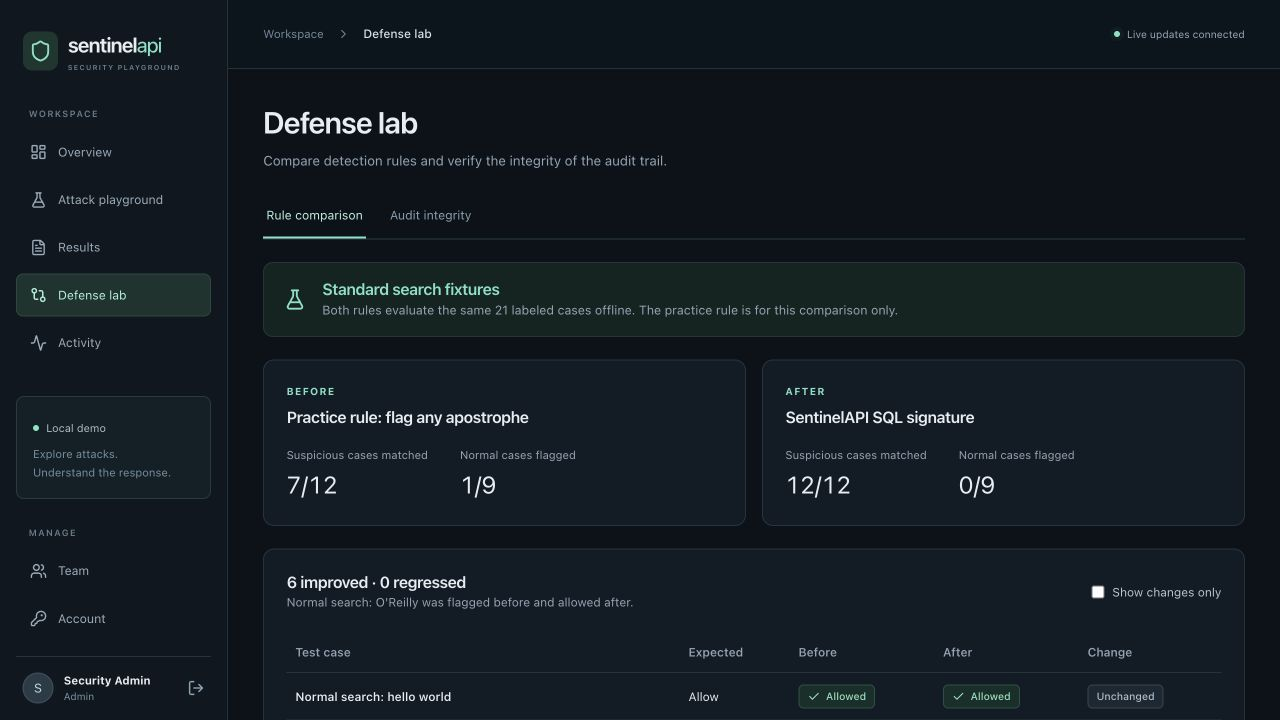
\includegraphics[width=.99\linewidth]{defense-lab.png}
\captionof{figure}{Defense Lab running locally. The screenshot shows the same fixed 21 cases evaluated by the practice rule and the current rule.}
\end{center}

\topic{Navigation used in the demonstration}
The Attack Playground is where an operator starts a scenario. Results shows past runs and exports. Defense Lab contains the rule comparison and audit verifier. Activity contains detections, incidents, sign-in history, and audit records.

\topic{Challenges and solutions}
The first visible flood response is not necessarily the first one the server processed. The grader reads the saved trigger evidence to identify the cooldown. The dashboard also reads old reports that predate the structured explanation fields; those reports show the responses and alerts they actually recorded.

\topic{How to use the screenshot}
The practice rule finds 7 of 12 suspicious cases and flags 1 of 9 normal cases. The current rule finds all 12 and flags none of the 9 normal cases. The surname row shows which false positive was corrected.


\chapter{Testing and security evaluation}
\section{Test design and expected results}
Each case declares its expected status and any required detector. Normal controls require no linked alert. The actual status remains visible when a case misses its evidence requirement.

\tabletitle{Standard profile case distribution}
\begin{tabularx}{\linewidth}{@{}>{\raggedright\arraybackslash}p{.26\linewidth}rY@{}}\toprule
\textbf{Scenario} & \textbf{Cases} & \textbf{Expected behavior}\\\midrule
Normal controls & 12 & 200, no alerts.\\
SQL injection & 12 & 403, SQL Injection evidence.\\
Cross-site scripting & 10 & 403, XSS evidence.\\
Path traversal & 6 & 403, Path Traversal evidence.\\
Command injection & 10 & 403, Command Injection evidence.\\
Password guessing & 20 & Early 401 responses, then 403 plus detector evidence.\\
Password spraying & 10 & Early 401 responses, then 403 plus detector evidence.\\
SSRF indicators & 8 & 403, restricted-host evidence.\\
Disguised upload & 4 & 403, file signature evidence.\\
Scanner headers & 6 & 403, scanner signature evidence.\\
Endpoint enumeration & 15 & 404, with a detector alert at 15.\\
Flood and recovery & 62 & 200/429 during the sequence, 200 on recovery.\\
\midrule
\textbf{Total} & \textbf{175} & \textbf{Response and case-linked evidence compared with the plan.}\\
\bottomrule\end{tabularx}

\topic{Negative controls}
Controls include normal search terms, apostrophes in names, nested but routine JSON, an ordinary upload, a valid demo login, and a public destination in simulated fetch. These cases make false positives measurable within the defined test set. The normal controls have their own profile selection for a quick local confidence check.

\sheet{Functional and authorization tests}
The checks cover startup, database health, access control, and whether saved records can be read again. The dashboard loading on its own does not show that the API can read or write PostgreSQL.

\tabletitle{Functional acceptance cases}
\bodytable{\textbf{Case} & \textbf{Expected observation}\\\midrule
Dashboard startup & Local interface loads and API health reports a connected database.\\
Account login & A valid account can open the dashboard. Invalid credentials return 401.\\
Viewer starts a run & Server refuses the action.\\
Report ownership & An analyst cannot retrieve another user's private report.\\
Alert review & Updating the verdict persists the value and creates an audit event.\\
Incident retrieval & Authorized user sees linked events. An unrelated analyst cannot read the incident.\\
Export & A saved experiment can produce a readable HTML, CSV, or JSON artifact.\\
Audit demo & Original sample verifies. An edited or truncated sample fails.\\}

\topic{Verification method}
The review and access checks ran in a separate local database schema with synthetic records. The checks used the owner, an unrelated analyst, a viewer, and an administrator. The verifier was also run against an edited record and a shortened trail in that schema.

\topic{What was freshly checked}
The verification checked that the verdict persisted, that status and verdict could differ, and that the incident timeline showed the review event. It also checked access to the audit verifier and opened the comparison, audit demo, and a saved incident. A later normal-case run generated signed events in the regular local database.

\sheet{Security and integrity checks}
Automated checks cover normalization, timer expiration, state isolation, and safe export. The integrity test also checks that two kinds of tampering fail verification.

\tabletitle{Security properties and why they are tested}
\bodytable{\textbf{Property} & \textbf{Verification idea}\\\midrule
Normalization & Recognized data inside supported encodings or a nested field reaches the appropriate rule.\\
Normal quotes & An ordinary apostrophe in a name remains accepted by the specific rule.\\
Counter boundary & Compare measures below the threshold and at the threshold. Confirm that the explanation uses the actual count.\\
Authorization & A viewer cannot label an alert. An unrelated analyst cannot cross the ownership boundary.\\
Evidence safety & Matched sensitive fields are redacted and exported values are encoded.\\
Audit changes & Verify an authentic sequence, then edit an old entry and remove the last entry in disposable data.\\}

\begin{lstlisting}[caption={Audit sample assertions based on tests/defense.test.ts}]
for (const change of ['edit', 'delete'] as const) {
  const result = demonstrateAuditIntegrity(change);
  assert.equal(result.original.valid, true);
  assert.equal(result.altered.valid, false);
}
\end{lstlisting}

Older events outside the signed range remain visible. The verifier reports them separately. Likewise, older simulation exports may lack fields that were introduced later. Open a recent run to see a recorded rule, field, or counter.

\sheet{Recorded timing}
A saved case includes the time from sending a request to receiving its reply. It includes work done before the API sent the reply. The full run time also includes the runner's overhead and any scheduled waits.

\tabletitle{Descriptive timing from archived reports}
\begin{tabularx}{\linewidth}{@{}Yrrrr@{}}\toprule
\textbf{Run} & \textbf{Median} & \textbf{P95} & \textbf{Max} & \textbf{Run time}\\\midrule
Standard, 175 cases & 2 ms & 6 ms & 13 ms & 31.569 s\\
Extended SQL and XSS, 142 cases & 2 ms & 2 ms & 3 ms & 0.398 s\\
Normal traffic, 12 cases & 3 ms & 12 ms & 12 ms & 0.065 s\\
\bottomrule\end{tabularx}

The table uses nearest-rank percentiles from the archived JSON. Each row describes one run. The Standard duration includes a 31-second recovery wait; the Extended duration covers only SQL and XSS. These elapsed times do not measure the isolated cost of a detector.

\topic{Overhead that matters}
The request timer combines parsing, authentication, detector checks, and any database writes before the reply. It cannot show which step costs the most. Dashboard updates and Guided pauses can add time outside that interval.

\topic{A fair follow-up benchmark}
A follow-up could repeat the same ordinary requests on one machine, with and without inspection and persistence. It should hold the database and runtime fixed, then report the spread across repetitions. Cooldown or teaching delays belong in the run duration, separately from request latency.

\sheet{Metrics and test procedure}
\topic{Expectation agreement}
Let $n$ be the number of completed cases eligible for comparison and $m$ the number satisfying the declared response and evidence rules.
\[
 \operatorname{Agreement} = \frac{m}{n}.
\]
This metric gives equal weight to each planned check. Some checks are linked, such as the attempts leading to a threshold and the subsequent recovery observation.

\topic{Classification metrics for labeled fixtures}
For the offline comparison, let TP be a suspicious case flagged, FP a normal case flagged, FN a suspicious case allowed, and TN a normal case allowed. Appropriate fixture metrics include
\[
 \operatorname{Recall}=\frac{\mathrm{TP}}{\mathrm{TP}+\mathrm{FN}},
 \qquad
 \operatorname{FPR}=\frac{\mathrm{FP}}{\mathrm{FP}+\mathrm{TN}}.
\]
An empty denominator gives an undefined rate. The offline corpus contains both positive and negative labels. It may overlap the patterns for which the rule was written, so the comparison is a regression exercise rather than an independent estimate.

\topic{Attribution gaps}
For Extended cases, the expected detector provides a reference label. A missing expected detector may occur when a case is allowed or when a different detector responds. The report keeps failed expectations, status counts, and connection errors separate, so a different 403 cannot be misread as proof that the intended detector worked.

\topic{Procedure followed}
The evaluation checked the build, lint, and tests, then read the profile and status totals from saved reports. The rule comparison and audit demonstration ran on fixed inputs. Ownership and state changes were checked separately with test records in a local database schema.

\chapter{Results}
\section{Standard run: HTTP outcomes}
The archived Standard run \texttt{509674dd} completed all 175 cases, and each met its planned status and evidence requirements \cite{artifacts}. The status counts show which accepted responses and rejections contributed to the total.

\tabletitle{Observed response distribution in the Standard run}
\begin{tabularx}{\linewidth}{@{}lrY@{}}\toprule
\textbf{Status} & \textbf{Count} & \textbf{Interpretation in the evaluated suite}\\\midrule
200 & 62 & Normal controls and rate-test responses accepted before limiting or after recovery.\\
401 & 8 & Initial incorrect demo logins across the guessing and spraying cases.\\
403 & 78 & Rejections from signature or behavioral detector rules.\\
404 & 15 & Missing routes. An enumeration alert was expected at the threshold.\\
429 & 12 & Rate-limited replies in the local flood experiment, including the cooldown check.\\
\midrule
Total & 175 & 175 expectations matched.\\
\bottomrule\end{tabularx}

All 12 normal controls returned 200 with no alert. The enumeration sequence returned 404 throughout and raised the expected alert at the threshold. Early invalid logins correctly returned 401. Counting only blocks would miss those successful tests.

\begin{lstlisting}[caption={An illustrative normal search used to explain the comparison}]
GET /search?q=O%27Reilly
Expected response: 200
Expected detector evidence: no alert
\end{lstlisting}

\topic{Provenance}
The Standard artifact was saved on 2 November 2026 in India Standard Time. It predates the Defense Lab update. Existing records can still be opened using saved evidence. Newly captured rule identifiers and counters are available from runs made after that update.

\topic{Reading the rate-limit result}
The 429 replies show when the local limit took effect. The 200 after the planned wait confirms recovery. This run provides no measure of traffic generated across multiple hosts.

\sheet{Extended run: missing detector evidence}
The saved two-family Extended run \texttt{c9ed9c0c} covered 142 SQL injection and XSS requests. The SQL cases accounted for 32 of the 36 unexpected results.

\tabletitle{Observed agreement by family in the selected Extended run}
\begin{tabularx}{\linewidth}{@{}Yrrrr@{}}\toprule
\textbf{Scenario} & \textbf{Cases} & \textbf{Matched} & \textbf{Unexpected} & \textbf{Agreement}\\\midrule
SQL injection & 72 & 40 & 32 & 55.6\%\\
Cross-site scripting & 70 & 66 & 4 & 94.3\%\\
\midrule
\textbf{Total} & \textbf{142} & \textbf{106} & \textbf{36} & \textbf{74.6\%}\\
\bottomrule\end{tabularx}

The server returned 34 HTTP~200 and 108 HTTP~403 replies. Only 106 cases met their expectations. A 403 from a different detector still counts as a missed attribution. The report records 36 missing attributions and zero transport errors.

\topic{Interpreting coverage}
Some corpus entries depend on how an application inserts the value into a query or page. A missed signature gives the team a case to review and possibly add to a regression set. The lab did not execute these inputs.

\topic{Limit of the result}
The 142-row artifact was saved on 26 October 2026. The planned full Extended suite contains 295 cases. The 74.6\% figure describes the selected two-family experiment and does not apply to the unmeasured full Extended plan.

\sheet{Before and after rule comparison}
The comparison uses 21 labeled search cases, comprising 12 suspicious cases and 9 normal cases. The practice rule flags any apostrophe. The application rule looks for more specific SQL signatures. Both rules receive the same extracted values.

\tabletitle{Confusion counts on the fixed comparison set}
\begin{tabularx}{\linewidth}{@{}Yrr@{}}\toprule
\textbf{Outcome} & \textbf{Practice rule} & \textbf{Application rule}\\\midrule
True positives & 7 & 12\\
False negatives & 5 & 0\\
False positives & 1 & 0\\
True negatives & 8 & 9\\
\midrule
Correct fixture decisions & 15/21 & 21/21\\
Suspicious-case recall & 58.3\% & 100.0\%\\
Normal-case false-positive rate & 11.1\% & 0.0\%\\
\bottomrule\end{tabularx}

Five previously missed suspicious cases were flagged, and the ordinary surname \texttt{O'Reilly} was allowed. No case went from matching its label to disagreeing with it. The comparison view highlights the six changed rows.

\topic{Why the comparison matters}
The SQL rule reduced both types of error on these cases. Testing suspicious examples alone would have missed the ordinary surname that the practice rule blocked.

\topic{Limits of the comparison}
The result describes the labeled fixture set. It does not show equal performance on independent traffic or all SQL contexts. The archived Extended run provides a separate example of why broader evaluation is needed. Future changes can reuse the same acceptance set and add independently labeled normal cases.

\sheet{Investigation and audit results}
\tabletitle{Verification performed after the Defense Lab update}
\bodytable{\textbf{Check} & \textbf{Observed result}\\\midrule
Backend and UI quality checks & Build and lint passed. All 12 automated tests passed.\\
New normal-traffic run & \texttt{a9fce53e}: all 12 cases returned 200 with no alert.\\
Review persistence & The isolated test saved a false-positive verdict, read it back, and checked its audit event.\\
Account access & Viewer write and out-of-scope analyst access were refused. Authorized access worked in the isolated test.\\
Live audit trail & Two newly signed events verified in the ordinary project database.\\
Tamper detection & An edit and a removed final event each failed verification in disposable data.\\}

\topic{Evidence an assessor can inspect}
Open a saved run, select its alert, and compare the response with the detector and review status. The incident timeline records when the analyst changed the verdict. The audit verifier checks whether the signed sequence still agrees with its checkpoint.

\topic{What the results support}
The isolated tests confirmed that a review record persists and that users cannot read outside their allowed scope. Audit verification passed for the original sample and failed for both modified copies. The table identifies which checks used disposable records and which used the regular database.

\chapter{Conclusion and future work}
\section{Conclusion and demonstration}
SentinelAPI shows what the API did, which rule made the decision, and what a reviewer did afterward. The enumeration case is a useful example: the API continues returning 404 after the detector has enough evidence to raise an alert.

The archived Standard suite matched all 175 expectations. The broader selected Extended suite produced 36 attribution gaps. The before-and-after comparison showed how a more specific rule removed one false positive and recognized five additional suspicious fixtures. The newer normal-traffic run confirmed ordinary request behavior after the investigation features were added.

\topic{Suggested classroom demonstration}
\begin{enumerate}
\item Open Defense Lab and use Show changes only. Explain the ordinary surname example.
\item Open a recent result and select Explain this decision. For a behavioral case, compare measurements below and at a threshold.
\item Open a saved incident and inspect linked alerts and investigator actions.
\item Show how recording a review verdict differs from resolving the alert.
\item Verify newly signed audit records, then run the disposable edit or deletion demonstration.
\end{enumerate}

\topic{Information security contribution}
Resolving an alert changes its workflow state. A separate verdict records the analyst's reason for closing it. The timeline makes that distinction visible, and audit verification checks whether the signed history of those actions still agrees with the checkpoint.

\sheet{Limitations and next steps}
\topic{Detection coverage}
Build an independently labeled set of ordinary and suspicious requests. Version the fixtures so later rules can be compared against the same examples. Review the 36 missed attributions in the selected Extended run before adding new conditions.

\topic{Deployment and measurement}
Counters are stored in one process. A deployment with several API processes would need shared state and a consistent way to identify a request source. Benchmark the current local setup before drawing conclusions about capacity.

\topic{Evidence integrity}
The signed range starts when audit signing is enabled. A checkpoint in separate write-restricted storage would help detect a rollback of the database and local checkpoint together. Key rotation would need to preserve verification of older signed records.

\topic{Investigation workflow}
Current timelines group events by run and linked alerts. A useful next step is to let analysts group related alerts across runs and save a note explaining why. Keep experiment fixtures distinct when reporting reviewer decisions.

\topic{Next evaluation milestone}
Run both profiles on the submission version and record its configuration. Keep the reports available for review. Test a wider set of normal inputs before making a claim about detection accuracy.

\renewcommand{\bibname}{References}
\begin{thebibliography}{99}
\addcontentsline{toc}{chapter}{References}
\small
\raggedright
\setlength{\itemsep}{.5em}
\bibitem{nist} K. Scarfone and P. Mell, \emph{Guide to Intrusion Detection and Prevention Systems (IDPS)}, NIST SP 800-94, 2007. \url{https://doi.org/10.6028/NIST.SP.800-94}.
\bibitem{owasp} OWASP Foundation, \emph{Web Security Testing Guide}, v4.2. \url{https://wstg.owasp.org/v4.2/4-Web_Application_Security_Testing/}.
\bibitem{bozic} J. Bozic and F. Wotawa, \emph{Planning-based security testing of web applications with attack grammars}, Software Quality Journal, vol. 28, pp. 307--334, 2020. \url{https://doi.org/10.1007/s11219-019-09469-y}.
\bibitem{brandi} C. Brandi, G. Perrone and S. P. Romano, \emph{Sniping at web applications to discover input-handling vulnerabilities}, Journal of Computer Virology and Hacking Techniques, vol. 20, pp. 641--667, 2024. \url{https://doi.org/10.1007/s11416-024-00518-0}.
\bibitem{penquest} R. Luh, M. Temper, S. Tjoa, S. Schrittwieser and H. Janicke, \emph{PenQuest: a gamified attacker/defender meta model for cyber security assessment and education}, Journal of Computer Virology and Hacking Techniques, vol. 16, pp. 19--61, 2020. \url{https://doi.org/10.1007/s11416-019-00342-x}.
\bibitem{mirage} M. Kouremetis et al., \emph{Mirage: cyber deception against autonomous cyber attacks in emulation and simulation}, Annals of Telecommunications, vol. 79, pp. 803--817, 2024. \url{https://doi.org/10.1007/s12243-024-01018-4}.
\bibitem{hmac} H. Krawczyk, M. Bellare and R. Canetti, \emph{HMAC: Keyed-Hashing for Message Authentication}, RFC 2104, 1997. \url{https://www.rfc-editor.org/info/rfc2104}.
\bibitem{http} R. Fielding, M. Nottingham and J. Reschke, eds., \emph{HTTP Semantics}, RFC 9110, 2022. \url{https://www.rfc-editor.org/info/rfc9110}.
\bibitem{rfc429} M. Nottingham and R. Fielding, \emph{Additional HTTP Status Codes}, RFC 6585, 2012. \url{https://www.rfc-editor.org/info/rfc6585}.
\bibitem{jwt} M. Jones, J. Bradley and N. Sakimura, \emph{JSON Web Token (JWT)}, RFC 7519, 2015. \url{https://www.rfc-editor.org/info/rfc7519}.
\bibitem{seclists} D. Miessler and contributors, \emph{SecLists}, repository and license. \url{https://github.com/danielmiessler/SecLists}. Pinned revision cited in Chapter 4.
\bibitem{artifacts} SentinelAPI project repository. Local implementation and archived run artifacts, including Standard run \nolinkurl{509674dd-9714-43ec-a701-b1db316f19c1}, Extended run \nolinkurl{c9ed9c0c-afd0-41d5-af37-91721ba5302b}, and normal run \nolinkurl{a9fce53e-f017-4148-bdf6-f37850cee805}. Defense Lab verification recorded in November 2026.
\end{thebibliography}
\end{document}

